\chapter{Ultrassom}

\section*{Introdução}

    \paragraph{}
    No capítulo de ultrassom iremos tratar dos ``olhos'' do \textit{Sparki}, eles estão presentes na plaquinha azul, naquilo que você pode ter considerado ser a cabeça dele. Embora, à primeira vista, os dois ``olhos'' pareçam câmeras feitas para que o nosso robozinho possua visão, na verdade eles fazem parte de um sensor bem diferente, que está mais associado com a \textbf{audição}. 

    Iremos então entender o que é esse sensor, como ele funciona e como podemos utilizá-lo facilmente, de forma que o \textit{Sparki} seja capaz de \textbf{desviar de obstáculos} enquanto anda.
    
\section{Sensor Ultrassônico}
    
    \begin{figure}[h]
    \caption{Imagem de um sensor ultrassônico}
     
    \centering 
    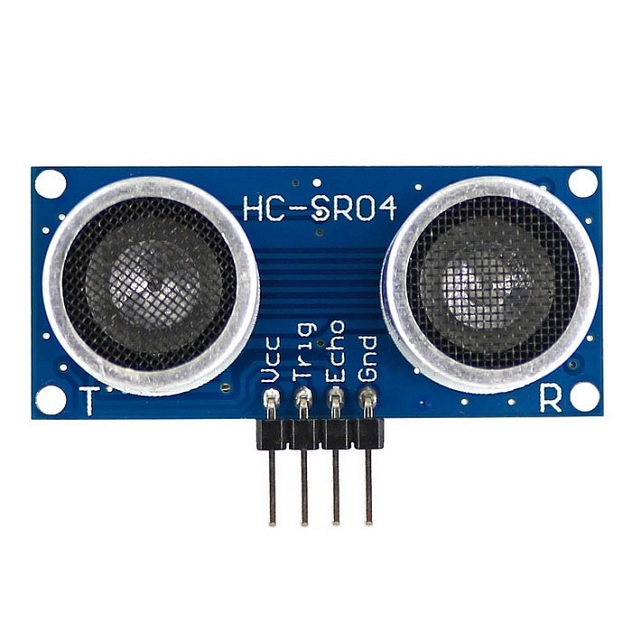
\includegraphics[width=3.5cm]{Figuras/ultrassom.jpg}
    \label{figura:ultrassom.jpeg}
    \end{figure}
    
    \paragraph{}
    O funcionamento do sensor é muito simples, o que muitos podem ter achado se tratar de duas câmeras na verdade são \textbf{um alto-falante e um microfone}. O alto-falante emite uma onda sonora de alta frequência, alta demais para que nós humanos sejamos capazes de escutá-la, essa onda de som é refletida assim que ela vai ao encontro a algum objeto e retorna para o microfone.
    \\~\\
    \textit{Mas qual a utilidade de se emitir um som e depois escutá-lo de volta?} \par
    A funcionalidade não está no som em si, mas sim no \textbf{tempo} que demorou para que a onda sonora retornasse para o sensor, essa informação de tempo é então utilizada para calcular a \textbf{distância do sensor até o objeto} que refletiu a onda de volta.
    
    \paragraph{}
    O sensor ultrassônico é utilizado para obtermos a distância entre o robô e algum objeto à sua frente. Mas nem sempre conseguimos encontrar essa distância como o esperado, isso ocorre pois às vezes o objeto não está bem posicionado, logo, ele não reflete o som de volta para o microfone, ou então ele absorve todo o som, isso pode acontecer se ele for muito macio.
    
    \begin{figure}[h]
    \caption{O objeto tem que se capaz de refletir a onda de volta para o microfone}
     
    \centering 
    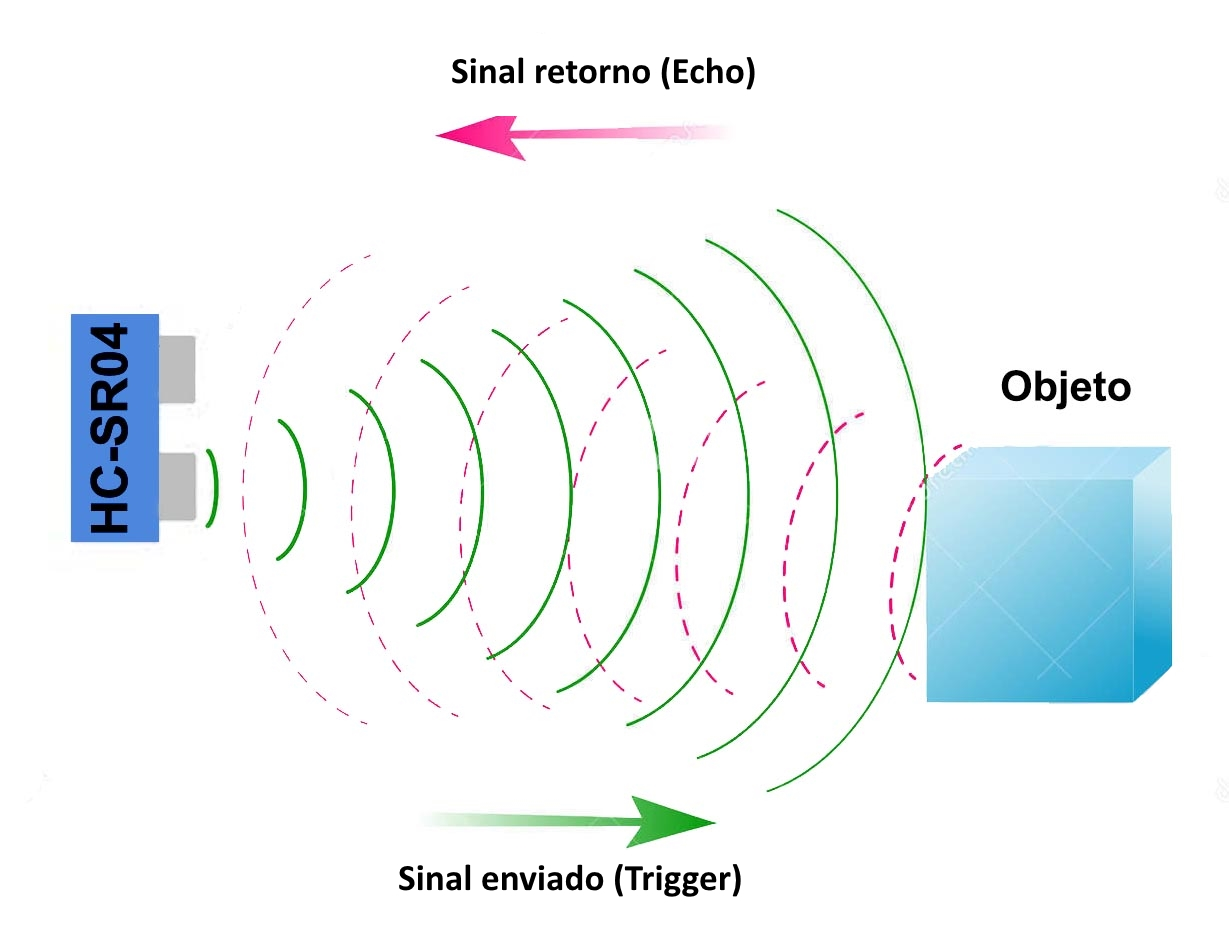
\includegraphics[width=7cm]{Figuras/onda.jpg}
    \label{figura:onda.jpeg}
    \end{figure}
    
\section{Aplicações no Cotidiano}

    \subsection*{Ultrassonografia}
    \paragraph{}
        A Ultrassonografia, também conhecida por Ecografia e Ultrassom, é um exame de diagnóstico que serve para visualizar em tempo real qualquer órgão ou tecido do corpo. Ela é comumente usada para observar o desenvolvimento do feto durante a gravidez. \par 
        Sabe aquelas imagens cinzas borradas que ninguém além do médico é capaz de compreender? Elas são feitas utilizando o ultrassom.
        
    \subsection*{Ecolocalização}
    \paragraph{}
        Embora não seja utilizada por seres humanos, a ecolocalização ou biossonar é muito importante na vida de diversos animais como morcegos, golfinhos e baleias. Eles são seres capazes de emitir ondas de alta frequência e cronometrar o tempo levado até que eles consigam escutar o seu próprio eco, assim, são capazes de conhecer seus arredores mesmo sem o uso da visão.
        
    \subsection*{Sonares}
    \paragraph{}
        Sonares são muito utilizados por navios e submarinos para detectar a presença de outros corpos debaixo da água, seu funcionamento é idêntico ao de um biossonar utilizado por uma baleia, por exemplo. Sonares diferem dos radares pois os radares utilizam ondas de rádio para medir a distância.
        
\section*{Função}

    \paragraph{}
    Para podermos utilizar o sensor ultrassônico presente no \textit{Sparki} tudo o que precisamos fazer é escrever a função \lstinline[columns=fixed]{sparki.ping()} que ela ativará o sensor. Como já dito, o sensor serve para medir a distância, logo, quando o ativamos, espera-se que recebamos algum valor de volta que indique qual é essa distância. Então, função \lstinline[columns=fixed]{sparki.ping()} já faz os cálculos necessários e nos \textbf{retorna} o valor da distância em \textbf{centímetros}.
    \\~\\
    \textit{A função então nos devolve um valor, mas como que eu vejo isso? Onde que ele vai me falar qual a distância que ele mediu? Ele escreve em algum lugar?} \par
    AHA! Acabamos de chegar na parte importante desse capítulo, as funções que retornam valores. O \textit{Sparki} irá escrever o valor que o sensor encontrou no local que a gente determinar para isso, mas claro que isso não quer dizer que podemos simplesmente falar para ele escrever a resposta num papel que ele irá fazer (possível, mas o código para isso seria muito grande). Uma forma interessante de resolver este conflito é a seguinte: nós criamos o local onde ele deve escrever a resposta, mas esse local não pode ser qualquer um, ele tem que ser uma \textbf{variável}. Sempre que criamos uma variável temos que definir também o tipo dela, e como, no nosso caso, estamos trabalhando apenas com centímetros é mais adequado criar uma variável do tipo \textbf{int}, ou seja, que armazena números inteiros.
    
    O código que mostra como fazemos isso está escrito logo abaixo:
    
\begin{lstlisting}[language=C]
#include <Sparki.h>;

int distancia_em_cm;

void setup()
{
}

void loop()
{
    distancia_em_cm = sparki.ping();  
    delay(300);
}
\end{lstlisting}

    Nesse código estamos dizendo que o \textit{Sparki} deve executar a função \lstinline[columns=fixed]{sparki.ping()} e salvar o valor que ela retornar dentro da nossa variável \lstinline[columns=fixed]{distancia_em_cm}. Agora que temos a nossa distância salva dentro de uma variável, podemos trabalhar com ela livremente para fazermos o que quiser, como fazer ele escrever o valor numa folha de papel.
    
    É importante notar a presença da função \lstinline[columns=fixed]{delay()} no código, pois o funcionamento do sensor não é tão rápido quanto a velocidade de processamento do nosso robô, então precisamos dar um pequeno intervalo de tempo para que o sensor possa funcionar sem erros.
    
\section{Servo motor}
    
    \paragraph{}
    Se considerarmos o sensor ultrassônico como sendo a ``cabeça'' do robô, é muito útil que tenhamos também um ``pescoço'' que sirva para movimentarmos a ``cabeça'', então surge a necessidade de um servo motor no \textit{Sparki}, mas afinal o que ele é?
    
    \begin{figure}[h]
    \caption{Imagem de um servo motor}
    
    \centering 
    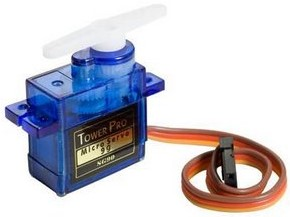
\includegraphics[width=9cm]{Figuras/servo.jpg}
    \label{figura:servo.jpeg}
    \end{figure}

    \paragraph{}
    Um servo motor é um motor que tem a capacidade de girar o seu eixo em ângulos precisos de até 90º ou 180º normalmente, sendo que o servo motor no qual o sensor ultrassônico está acoplado é capaz de girar seu eixo em até 180º. Ele é muito útil para movimentar braços robóticos, por exemplo. Nesse caso não é necessária a realização de voltas completas e a precisão torna-se muito importante. No nosso caso, utilizamos dele para girar o sensor e, assim, podermos medir distâncias em outras direções sem ter que utilizar as rodas para girar o robô, infelizmente não temos como fazer o \textit{Sparki} olhar para cima ou para baixo utilizando um servo motor apenas.
    
\subsection{Função}

    \paragraph{}
    Agora que sabemos da existência do servo motor, precisamos saber como utilizá-lo. Para começar, devemos ativá-lo escrevendo a função \lstinline[columns=fixed]{sparki.servo()}, esta função deve receber um valor de angulação em graus, que determina o quanto ele deve girar, este valor deve estar entre -90º e 90º (sendo valores negativos para a esquerda e positivos para a direita) e o valor pode ser um número quebrado, isto é, o argumento da função é do tipo \textbf{float}.
    
    \paragraph{}
    Para facilitar a nossa vida, a função \lstinline[columns=fixed]{sparki.servo()} já vem com 3 valores predefinidos dos ângulos mais utilizados: SERVO\underline{\hspace{.1in}}LEFT (-90º),  SERVO\underline{\hspace{.1in}}CENTER (0º) e SERVO\underline{\hspace{.1in}}RIGHT (90º), assim tudo o que precisamos fazer é escrever SERVO\underline{\hspace{.1in}}| com o sentido desejado como argumento que o \textit{Sparki} se encarrega de colocar o sensor na posição correta.
    \\~\\
    Abaixo temos um código que faz com que o \textit{Sparki} meça a distância dele para os objetos na sua esquerda, frente, direita e diagonais esquerda e direita.

\begin{lstlisting}[language=C]
#include <Sparki.h>;

int distancia_esquerda, distancia_direita, distancia_frente,
distancia_diagonal_esquerda, distancia_diagonal_direita;

void setup()
{
    sparki.servo(SERVO_LEFT);   //gira para a posição -90 graus
    delay(500)
    distancia_esquerda = sparki.ping();  
    delay(500);
    sparki.servo(-45);   //gira para a posição -45 graus
    delay(500)
    distancia_diagonal_esquerda = sparki.ping();  
    delay(500);
    sparki.servo(SERVO_CENTER);   //gira para a posição 0 graus
    delay(500)
    distancia_frente = sparki.ping();  
    delay(500);
    sparki.servo(45);   //gira para a posição 45 graus
    delay(500)
    distancia_diagonal_direita = sparki.ping();  
    delay(500);
    sparki.servo(SERVO_RIGHT);   //gira para a posição 90 graus
    delay(500)
    distancia_direita = sparki.ping();  
    delay(500);
}

void loop()
{
}
\end{lstlisting}    
    

\section{Exercícios}

    \question{Responda a seguinte pergunta: como podemos encontrar a distância até um objeto utilizando apenas as informações do tempo que a onda de alta frequência demorou para retornar ao sensor e a velocidade dessa mesma onda?}
    
    \begin{center}
        \line(1,0){450}
        \vspace{0.2cm}   
        \line(1,0){450}
        \vspace{0.2cm}   
        \line(1,0){450}
        \vspace{0.2cm} 
        \line(1,0){450}
        \vspace{0.4cm} 
    \end{center}

    \question{Com os conhecimentos adquiridos até agora, escreva um pequeno código que mostre a todo momento na tela LCD a distância do \textit{Sparki} até algum objeto que esteja na sua frente.}

    \begin{center}
        \line(1,0){450}
        \vspace{0.2cm}   
        \line(1,0){450}
        \vspace{0.2cm}   
        \line(1,0){450}
        \vspace{0.2cm}   
        \line(1,0){450}
        \vspace{0.2cm}   
        \line(1,0){450}
        \vspace{0.4cm} 
    \end{center}
    
    \question{Escreva um código que centre o sensor ultrassônico quando o \textit{Sparki} é ligado e que depois de 3 segundos faça ele ficar balançando o sensor de um lado para o outro.}
    
    \begin{center}
        \line(1,0){450}
        \vspace{0.2cm}   
        \line(1,0){450}
        \vspace{0.2cm}   
        \line(1,0){450}
        \vspace{0.2cm}   
        \line(1,0){450}
        \vspace{0.2cm}   
        \line(1,0){450}
        \vspace{0.4cm} 
    \end{center}

    \question{Escreva um código que faça com que o \textit{Sparki} determine a distância até o objeto logo a sua frente e então ande na direção dele e pare a 7cm de distância do objeto.}

    \begin{center}
        \line(1,0){450}
        \vspace{0.2cm}   
        \line(1,0){450}
        \vspace{0.2cm}   
        \line(1,0){450}
        \vspace{0.2cm}   
        \line(1,0){450}
        \vspace{0.2cm}   
        \line(1,0){450}
        \vspace{0.4cm} 
    \end{center}
    
    \challenge{\large{Desafio: Escreva um código onde o \textit{Sparki} gira em até 360º e então mostra na tela LCD as distâncias dos objetos a sua volta nas direções norte, nordeste, leste, sudeste, sul, sudoeste, oeste e noroeste.}}
    
    \begin{center}
        \line(1,0){450}
        \vspace{0.2cm}   
        \line(1,0){450}
        \vspace{0.2cm}   
        \line(1,0){450}
        \vspace{0.2cm}   
        \line(1,0){450}
        \vspace{0.2cm}   
        \line(1,0){450}
        \vspace{0.4cm} 
    \end{center}